\documentclass[]{article}
\usepackage{lmodern}
\usepackage{amssymb,amsmath}
\usepackage{ifxetex,ifluatex}
\usepackage{fixltx2e} % provides \textsubscript
\ifnum 0\ifxetex 1\fi\ifluatex 1\fi=0 % if pdftex
  \usepackage[T1]{fontenc}
  \usepackage[utf8]{inputenc}
\else % if luatex or xelatex
  \ifxetex
    \usepackage{mathspec}
  \else
    \usepackage{fontspec}
  \fi
  \defaultfontfeatures{Ligatures=TeX,Scale=MatchLowercase}
\fi
% use upquote if available, for straight quotes in verbatim environments
\IfFileExists{upquote.sty}{\usepackage{upquote}}{}
% use microtype if available
\IfFileExists{microtype.sty}{%
\usepackage{microtype}
\UseMicrotypeSet[protrusion]{basicmath} % disable protrusion for tt fonts
}{}
\usepackage[margin=1in]{geometry}
\usepackage{hyperref}
\hypersetup{unicode=true,
            pdftitle={CPR Report Card},
            pdfborder={0 0 0},
            breaklinks=true}
\urlstyle{same}  % don't use monospace font for urls
\usepackage{graphicx,grffile}
\makeatletter
\def\maxwidth{\ifdim\Gin@nat@width>\linewidth\linewidth\else\Gin@nat@width\fi}
\def\maxheight{\ifdim\Gin@nat@height>\textheight\textheight\else\Gin@nat@height\fi}
\makeatother
% Scale images if necessary, so that they will not overflow the page
% margins by default, and it is still possible to overwrite the defaults
% using explicit options in \includegraphics[width, height, ...]{}
\setkeys{Gin}{width=\maxwidth,height=\maxheight,keepaspectratio}
\IfFileExists{parskip.sty}{%
\usepackage{parskip}
}{% else
\setlength{\parindent}{0pt}
\setlength{\parskip}{6pt plus 2pt minus 1pt}
}
\setlength{\emergencystretch}{3em}  % prevent overfull lines
\providecommand{\tightlist}{%
  \setlength{\itemsep}{0pt}\setlength{\parskip}{0pt}}
\setcounter{secnumdepth}{0}
% Redefines (sub)paragraphs to behave more like sections
\ifx\paragraph\undefined\else
\let\oldparagraph\paragraph
\renewcommand{\paragraph}[1]{\oldparagraph{#1}\mbox{}}
\fi
\ifx\subparagraph\undefined\else
\let\oldsubparagraph\subparagraph
\renewcommand{\subparagraph}[1]{\oldsubparagraph{#1}\mbox{}}
\fi

%%% Use protect on footnotes to avoid problems with footnotes in titles
\let\rmarkdownfootnote\footnote%
\def\footnote{\protect\rmarkdownfootnote}

%%% Change title format to be more compact
\usepackage{titling}

% Create subtitle command for use in maketitle
\providecommand{\subtitle}[1]{
  \posttitle{
    \begin{center}\large#1\end{center}
    }
}

\setlength{\droptitle}{-2em}

  \title{CPR Report Card}
    \pretitle{\vspace{\droptitle}\centering\huge}
  \posttitle{\par}
    \author{}
    \preauthor{}\postauthor{}
    \date{}
    \predate{}\postdate{}
  
\usepackage{floatrow}

\begin{document}
\maketitle

\newfloatcommand{btabbox}{table}

\begin{figure}[H]
  \begin{floatrow}
    \ffigbox{%

\begin{flushright}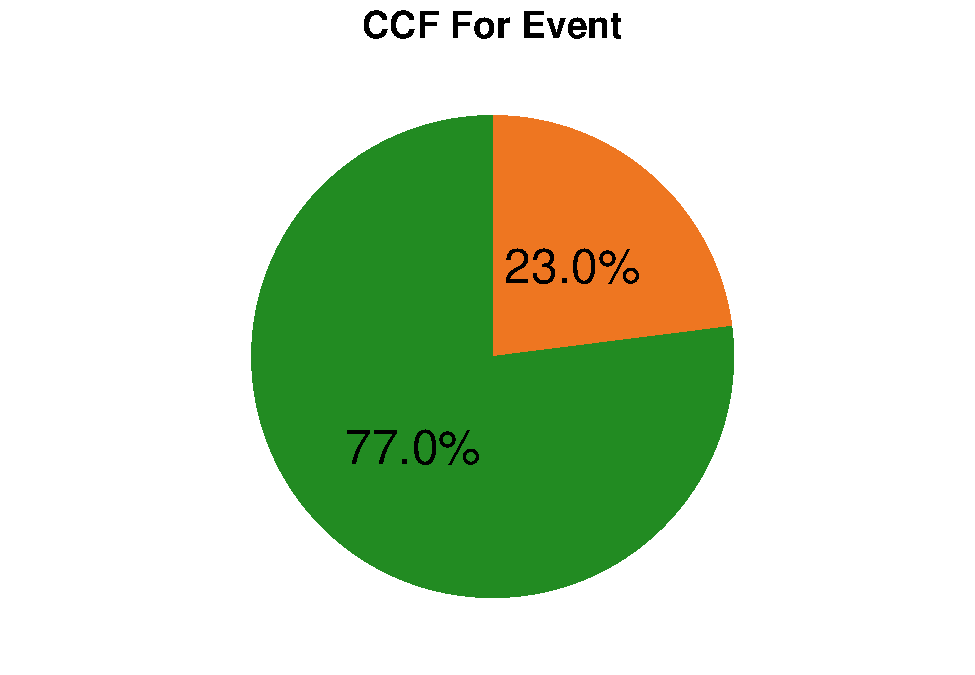
\includegraphics{report_files/figure-latex/unnamed-chunk-1-1} \end{flushright}
    }{\caption{CCF Pie Chart}}

    \btabbox{%

\begin{tabular}{l|l}
\hline
Event CCF Metrics & \\
\hline
CCF (\%) & 65.26\%\\
\hline
(\%) Not in CCs & 34.74\%\\
\hline
Total CCs (n) & 1374\\
\hline
Total Time of Event (min) & 64.5\\
\hline
\end{tabular}
    }{\caption{CCF Table}}
  \end{floatrow}
\end{figure}

\begin{figure}[H]
  \begin{floatrow}
    \btabbox{%

\begin{tabular}{l|l}
\hline
Event Average Depth \& Rate & \\
\hline
Depth (cm) & 4.2\\
\hline
Rate (cpm) & 125.6\\
\hline
\end{tabular}
    }{\caption{Average Table}}
    
     \btabbox{%

\begin{tabular}{l|l}
\hline
 & Percentage\\
\hline
Compressions in Target Depth: & 36\%\\
\hline
Compressions in Target Rate: & 19\%\\
\hline
\end{tabular}
   }{\caption{Percent Table}}
  \end{floatrow}
\end{figure}

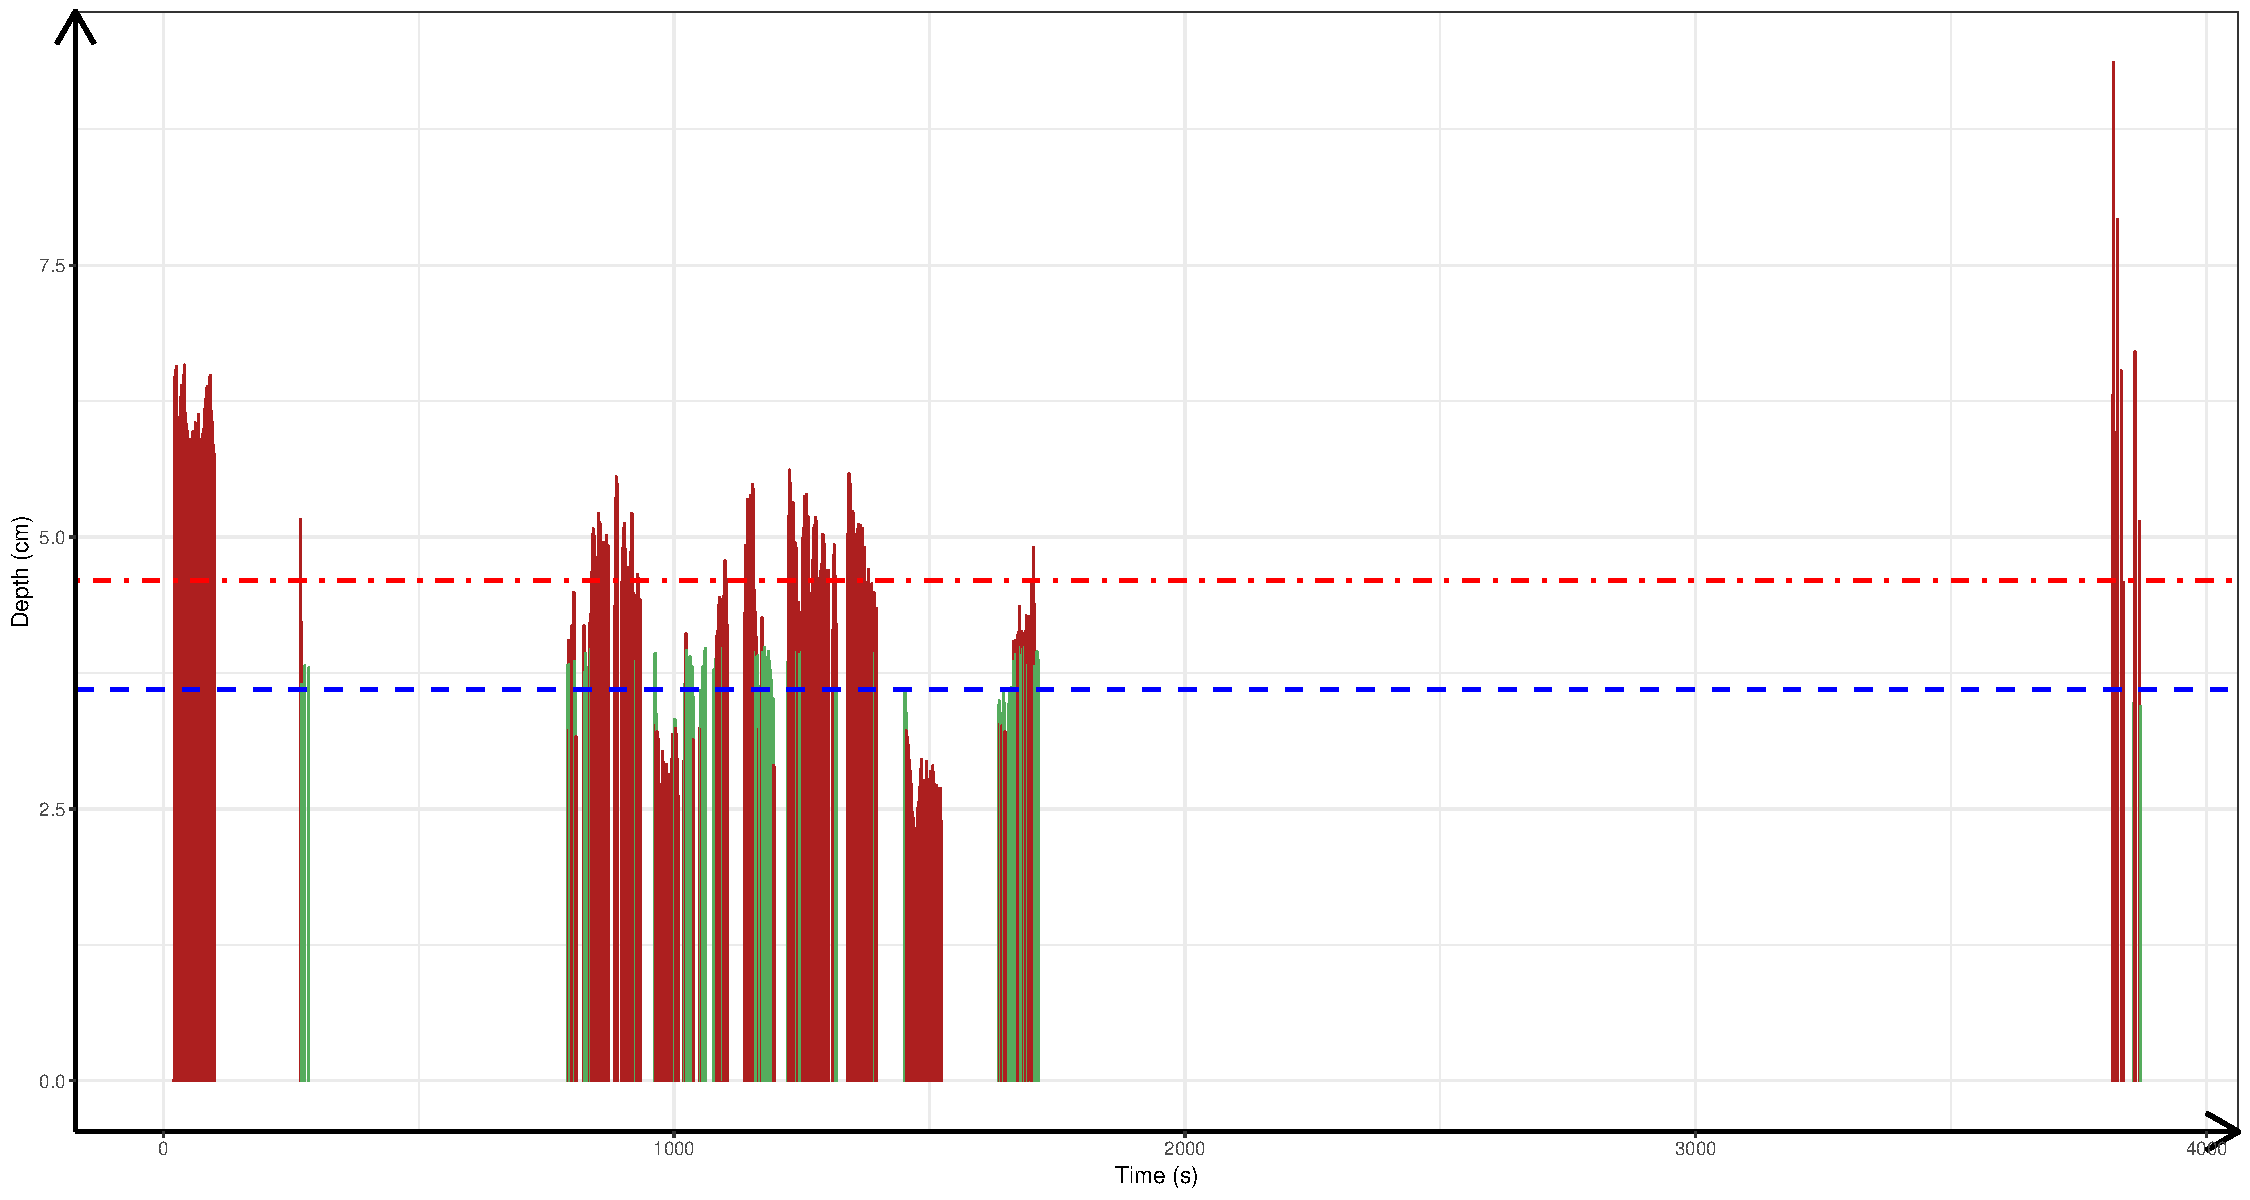
\includegraphics{report_files/figure-latex/depth plot-1.pdf}

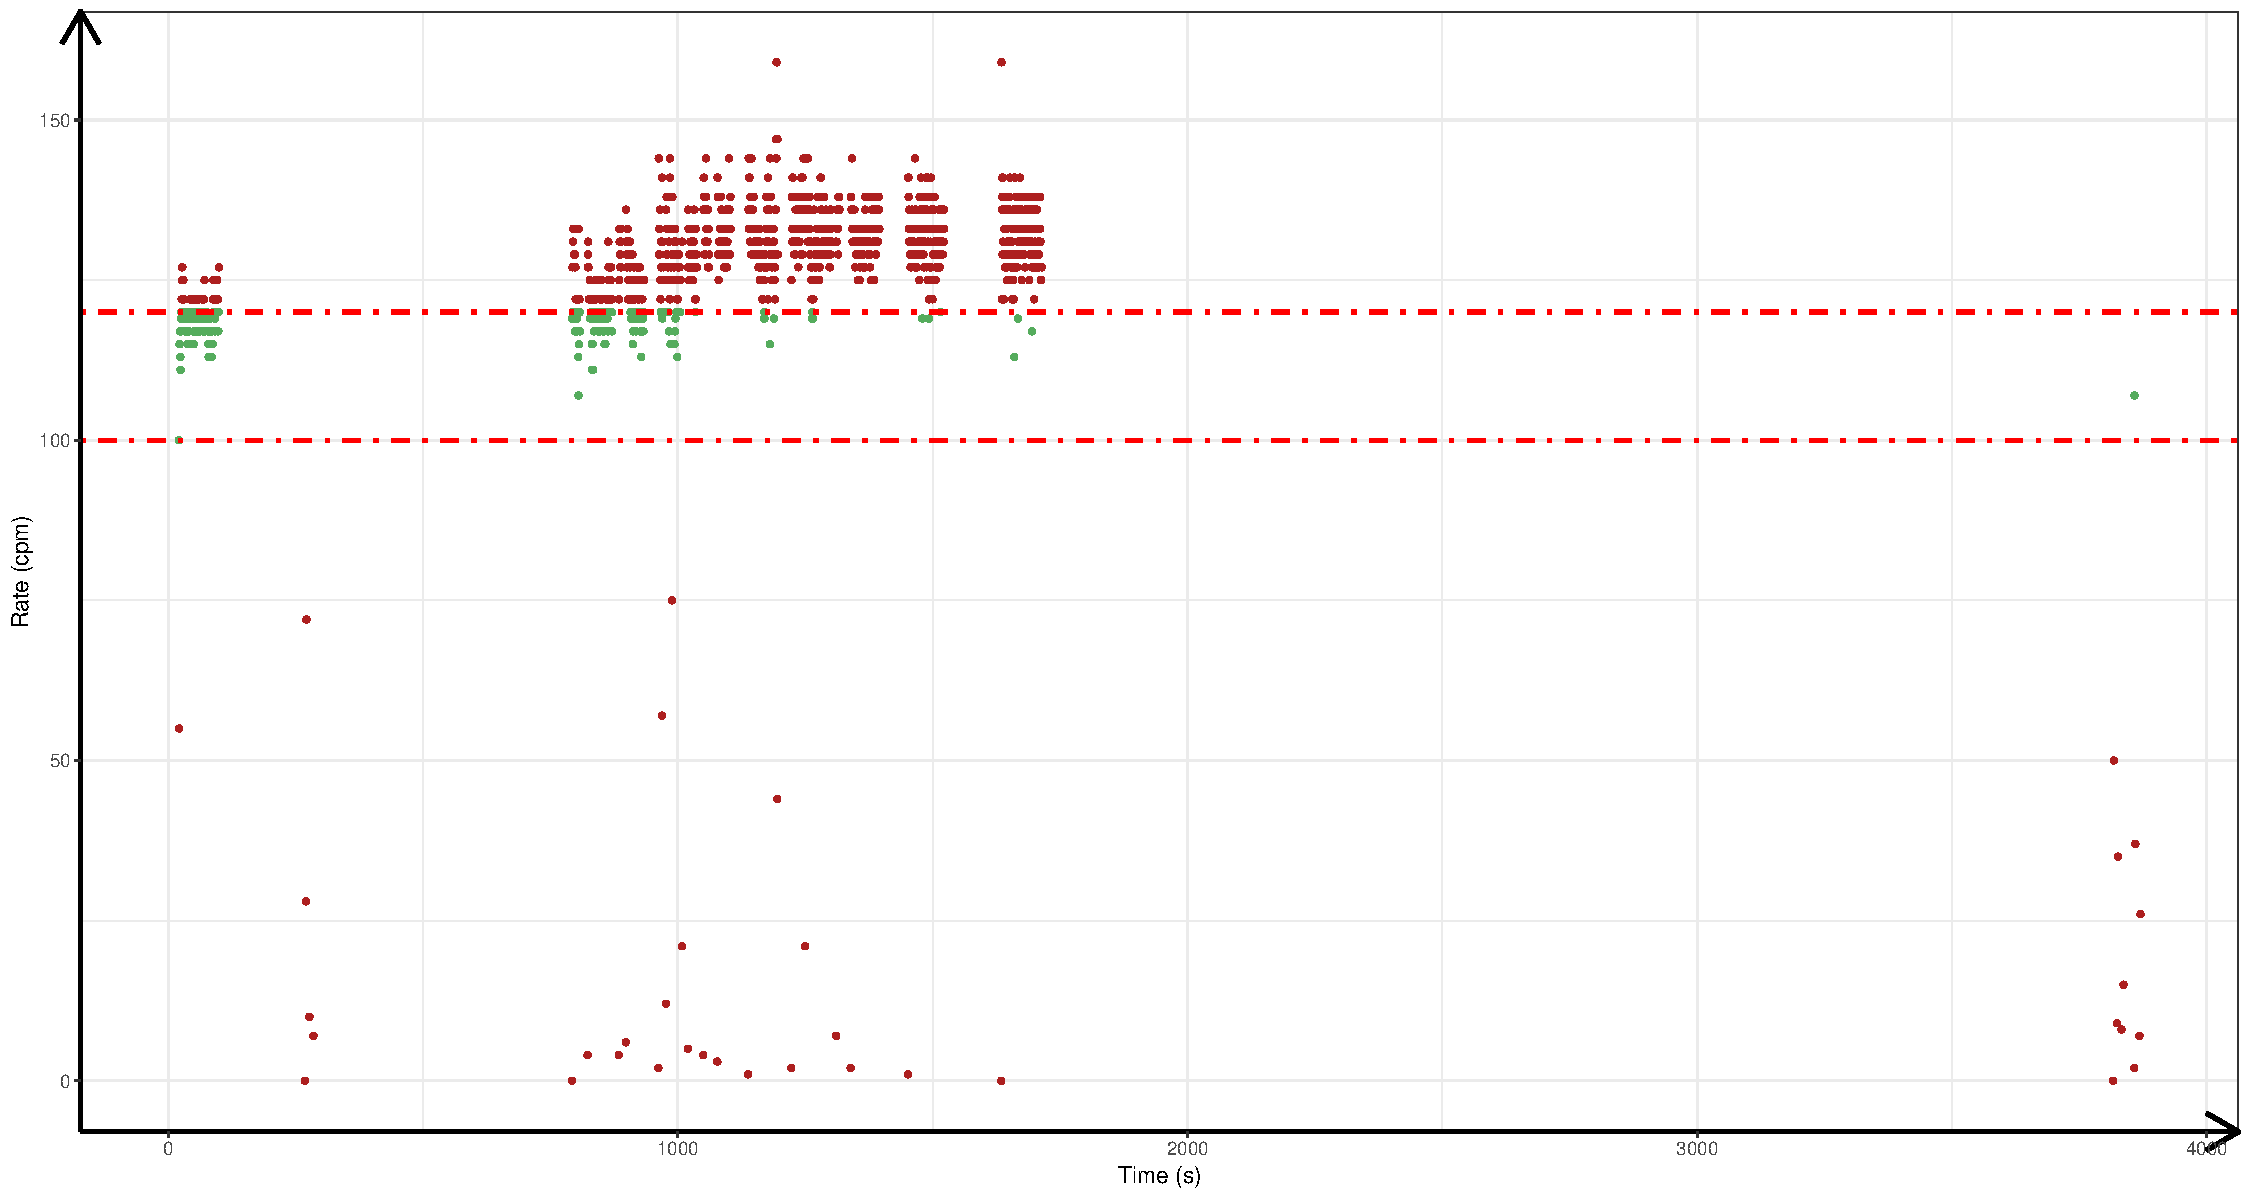
\includegraphics{report_files/figure-latex/rate plot-1.pdf}


\end{document}
